\chapter{Internet}
\label{ch:internet}

The \textbf{Internet} is a 60 years old project that still has legacy elements from its original implementation - an incredibly long time for a telecommunication network. It was built slowly, piece by piece, as it was initially developed for small, monolithic networks (that evolved based on what vendors wanted), and thus it was dramatically difficult to use.

Internet survived and thrived because of many factors, among which we can find:

\begin{itemize}
    \item \textbf{economical} factors: it was and still is (almost) free;
    \item \textbf{technological} factors: it was open, so anyone could devise their own protocols;
    \item \textbf{ease of use}: it was a lot  simpler than using raw sockets;
    \item \textbf{final users}: they were the same as the developers, so they could change whatever did not work as they wanted it to;
    \item \textbf{political} factors: telecommunications companies have driven all wireless and wired standards, even though they thought for a (too) long time that traditional communications (phone calls, SMS) were better.
\end{itemize}

The one thing that has always hindered (and probably always will) the Internet's development is the fact that it has to cope with everything that has already been rolled out (like the TCP/IP protocol), making it difficult to widespread new, better protocols.

%----------------------------------------------------------------------------------------

\section{History of Internet}
A detailed history of the Internet\footnote{Wikipedia, \textit{\url{http://en.wikipedia.org/wiki/Internet}}} and protocols like the one mentioned above\footnote{Wikipedia, \textit{\url{https://en.wikipedia.org/wiki/Internet\_protocol\_suite}}} can be easily found, well, on the Internet itself. It mostly consists of continuous attacks and attempts from companies and governments to make them their own, although fortunately nobody really succeeded.

Until the 70s, the Internet underwent a basic technical evolution, and vertical network models\footnote{\textbf{Vertical networks} connect people who have very specific interests. To be considered a vertical network, the focus of that group must be a specific niche.} were mostly used.

During the 80s and 90s the Internet became known to the world, and services began to be available to everyone. Competition between service providers started in those years.

Nowadays, the Internet is omnipresent and offers thousands of different services both legal or illegal; for this reason, it is often restricted by politics and economics. Net neutrality has become an important principle that many people advocate for.

%----------------------------------------------------------------------------------------

\section{What is the Internet made of?}
\label{sec:internetmadeof}
The Internet is not a single network, but an \textbf{interconnection of networks} and a collection of autonomous systems. It is based on \textbf{Request for Comments}, or \textbf{RFC}s, publications from the Internet Society (ISOC) and its associated bodies (like the Internet Engineering Task Force (IETF)), the main technical development and standards-setting bodies for the Internet. A RFC is authored by individuals or groups of engineers and computer scientists in the form of a memorandum describing methods, behaviors, research, or innovations applicable to the workings of the Internet and Internet-connected systems. It is submitted either for peer review or to convey new concepts, information, or occasional engineering humor.

Clearly, the physical host connections of the Internet are not as important as the protocols that make communication possible; although the Internet is based on TCP/IP, there are tons of other different protocols, and TCP/IP itself is very flexible (it can be applied in a lot of ways, including using actual birds\footnote{\label{foot:birds}\textbf{RFC 1149}, \textit{A Standard for the Transmission of IP Datagrams on Avian Carriers};\\\textbf{RFC 2549} \textit{IP over Avian Carriers with Quality of Service};\\ \textbf{RFC 6214} \textit{Adaptation of RFC 1149 for IPv6}.}).

%-------------------------------------------

\subsection{Internet mapping}

\begin{figure}[H]
  \centering
  \begin{minipage}[b]{0.4\textwidth}
    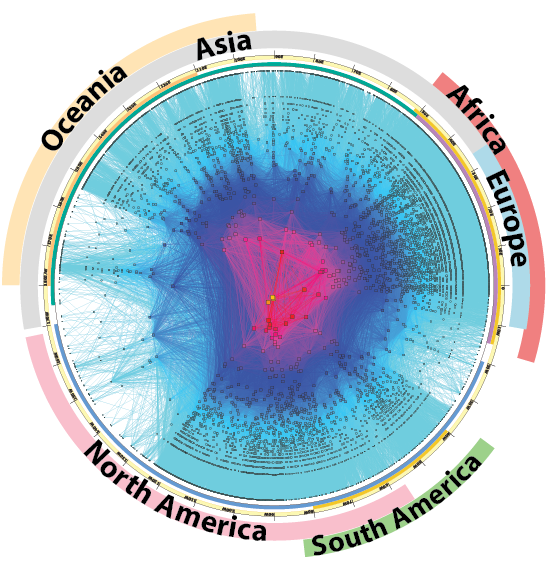
\includegraphics[scale=0.35]{img/caida2015.png}
    \decoRule
    \caption{CAIDA IPv4 2015 Internet map.}
    \label{fig:caida2015}
  \end{minipage}
  \hfill
  \begin{minipage}[b]{0.4\textwidth}
    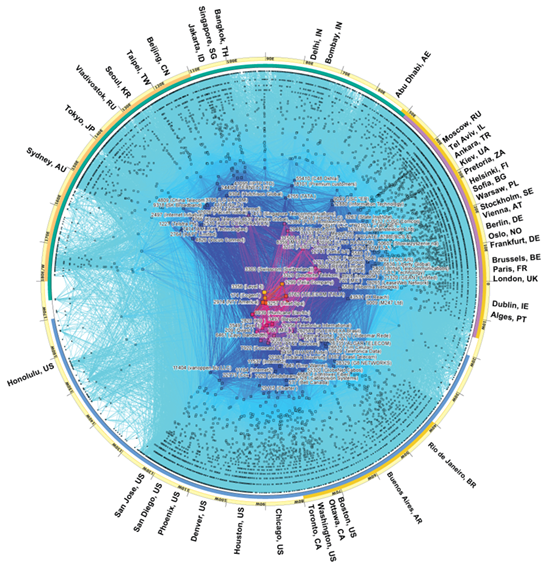
\includegraphics[scale=0.35]{img/caida2017.png}
    \decoRule
    \caption{CAIDA Ipv4 2017 Internet map.}
    \label{fig:caida2017}
  \end{minipage}
\end{figure}

Many organizations such as the Center for Applied Internet Data Analysis (\textbf{CAIDA}) perform \textbf{Internet mapping}, which is the study of the physical connectivity of the Internet. They collect, monitor, analyze, and visualize several forms of Internet traffic data concerning network topology, which is used for a variety of applications in business and society.

For example, in the CAIDA maps shown below (figures \ref{fig:caida2015} and \ref{fig:caida2017}), every dot is an autonomous system like a blob of routers, computers (thus not a single network node like a computer or a router), and is central or peripheral depending on how much traffic it generates or receives. Two dots are connected by a line if they exchange data directly, while red lines are Internet superhighways, which carry more traffic and are usually different from final users' lines.

%-------------------------------------------

\subsection{Some definitions}
Key principle: \textbf{K.I.S.S.}, \textit{Keep It Simple and Stupid}. Many things are hidden and/or simplified for our own safety.

%----------------------

\subsubsection*{Autonomous system}
Collection of connected Internet Protocol (IP) routing prefixes under the control of one or more network operators that presents a common, clearly defined routing policy to the Internet\footnote{RFC 1930, section 3.}. An AS is different from a subnet, as it is a management concept; any security policy at level of routing/network must be done into an autonomous system, and different autonomous systems will have different policies. There is no central authority that can tell an AS what policies to implement, because - like the name implies - they are autonomous.

%----------------------

\subsubsection*{Gateway}
Network entity also called the protocol converter. It can connect a computer of one network to another and defines the boundaries of a network; like a router, is an intermediate node which requires an IP interface for each subnet it is connected to. It resides in the third and/or seventh layer of the ISO/OSI protocol stack.

%----------------------

\subsubsection*{Host}
The source and destination of data, which must be uniquely identified by its IP address. It resides in the third layer of the ISO/OSI protocol stack.

%----------------------

\subsubsection*{Network}
Medium to which many nodes can be connected, on which every node has an address and which permits nodes connected to it to transfer messages to other nodes connected to it by merely providing the content of a message and the address of the destination node, then letting the network find the way to deliver the message to the destination node, possibly routing it through intermediate nodes.

%----------------------

\subsubsection*{Protocol stack}
Group of protocols that all work together to allow software or hardware to perform a function. In telecommunications, the TCP/IP protocol stack is a good example.

%----------------------

\subsubsection*{Router}
Network device that connects multiple networks together and controls the data traffic between them. A router is an intermediate node which needs an IP interface for each subnet it is connected to and, based on internal routing tables, it reads each incoming packet’s IP address and its destination IP address, then decides the shortest possible path to forward it after guessing the destination subnet (magic applies here):

\begin{itemize}
    \item if the destination is on a subnet directly connected to the router, it sends the packet directly;
    \item otherwise, finds the best next router and sends the packet to it.
\end{itemize}

Every router makes decisions on its own; this idea was developed in an attempt to make routers self-recovering. It resides in the third and/or seventh layer of the ISO/OSI protocol stack.

%----------------------

\subsubsection*{Routing table}
List of IP addresses that a router can connect to in order to transfer data.

%----------------------

\subsubsection*{Service Access Point (SAP)}
Identifying label for network endpoints used in ISO/OSI networking. Basically, the SAP is a conceptual location at which one ISO/OSI layer can request the services of another ISO/OSI layer.

%----------------------

\subsubsection*{Subnet}
Segment of a network identified by a \textit{\{Network Address\footnote{A \textbf{network address} is an identifier for a node or host on a telecommunications network.}, Subnet Mask}\} pair; it basically is a network inside a network. Through subnetting, network traffic can travel a shorter distance without passing through unnecessary routers to reach its destination, while routers are used to communicate between different subnets.

%----------------------

\subsubsection*{Subnet mask}
Similar to an IP address, but for only internal usage within a subnet. It is not indicated within data packets traversing the Internet, because those packets only indicate the destination IP address.

%----------------------------------------------------------------------------------------

\section{Structure of Internet}
How much should we know about Internet protocols? Nothing, and everything: a lot of security issues are strictly related to a protocol and how it works. In order to know or find vulnerabilities of a protocol we need to know it very well (not just because we studied it, but because we dissected it like a frog), even better than the person who devised it. However, we cannot ask anybody to know every single protocol that has ever been developed: the goal of this course is to teach what are the most important vulnerabilities, and a few things about how to find new ones. Mostly, in the end we should be able to know what to look for and where to get our hands dirty.

The idea behind the main Internet protocol stack model, the ISO/OSI model, is to divide the network in many separated layers, where the $n$-th layer offers services to the $(n+1)$-th layer and receives services from the $(n-1)$-th layer, each at their own SAP (fig. \ref{fig:layers_idea}). Note that if protocol $n$ communicates with a different layer on another device (one that is not an equivalent of layer $n$), then whoever devised it is either an idiot or a genius (most likely an idiot): this should \textit{never} happen.

\begin{figure}[H]
    \centering
    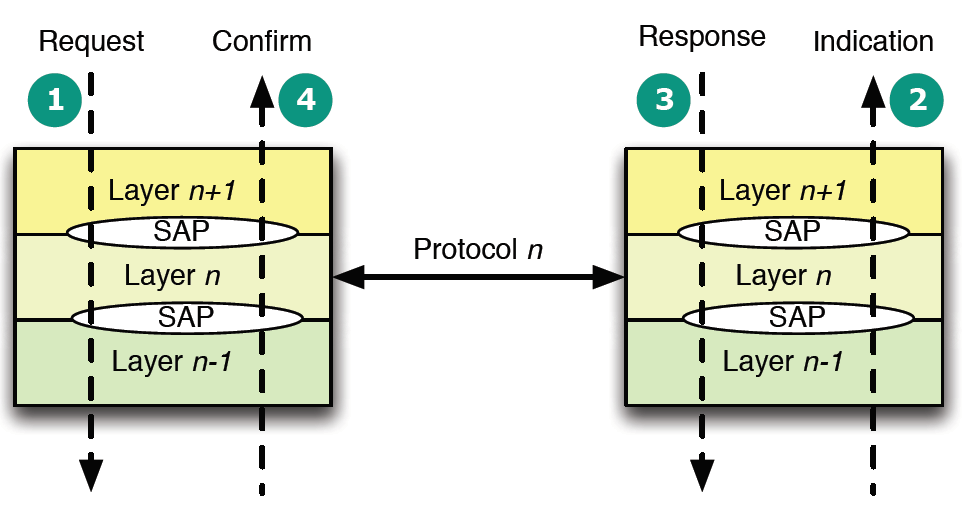
\includegraphics[scale=0.5]{img/layers_idea.png}
    \decoRule
    \caption{ISO/OSI model layer communication.}
    \label{fig:layers_idea}
\end{figure}

%----------------------

\subsubsection*{PDU and encapsulation}
In a network protocol made up of several layers each layer adds its own data in a header and (optionally) a trailer by building a \textbf{Protocol Data Unit} (PDU), as shown in figure \ref{fig:pdu}. The principle followed is that of \textbf{encapsulation}, a method of designing modular communication protocols in which logically separate functions in the network are abstracted from their underlying structures by inclusion or information hiding within higher level objects (see example in fig. \ref{fig:udp_pdu}).

Encapsulation is:

\begin{itemize}
    \item \textbf{recursive}: each layer adds its own header (and trailer, if any);
    \item \textbf{reversible}: it is always possible to correctly de-encapsulate the PDU of the layer above.
\end{itemize}

\begin{figure}[H]
    \centering
    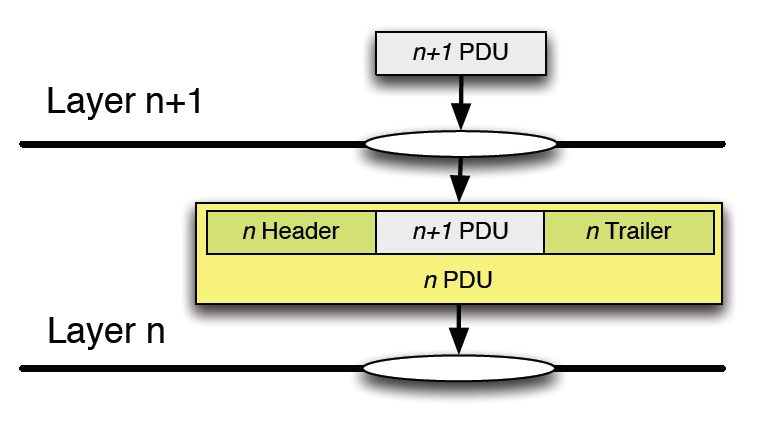
\includegraphics[scale=0.5]{img/pdu.png}
    \decoRule
    \caption{Protocol Data Unit (PDU) and encapsulation.}
    \label{fig:pdu}
\end{figure}

\begin{figure}[H]
    \centering
    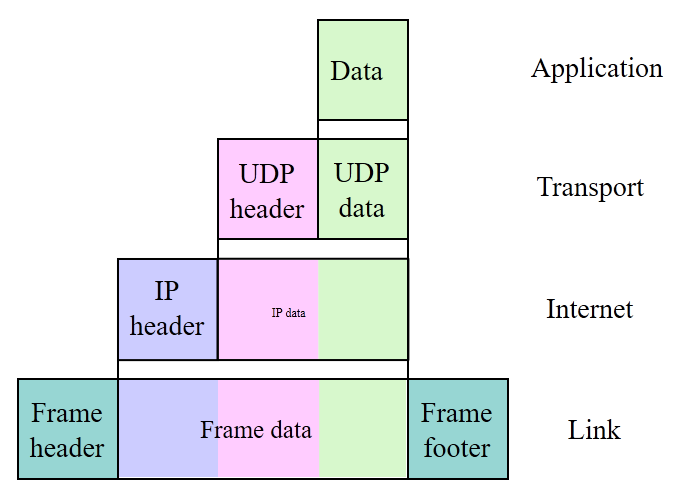
\includegraphics[scale=0.5]{img/udp_pdu.png}
    \decoRule
    \caption{An example of encapsulation of user data in the User Datagram Protocol (UDP) stack, in which each new layer includes the data from the previous layer, but without being able to identify which part of the data is the header or trailer from the previous layer. This effectively hides (encapsulates) the information from lower layers.}
    \label{fig:udp_pdu}
\end{figure}

\begin{figure}[H]
    \centering
    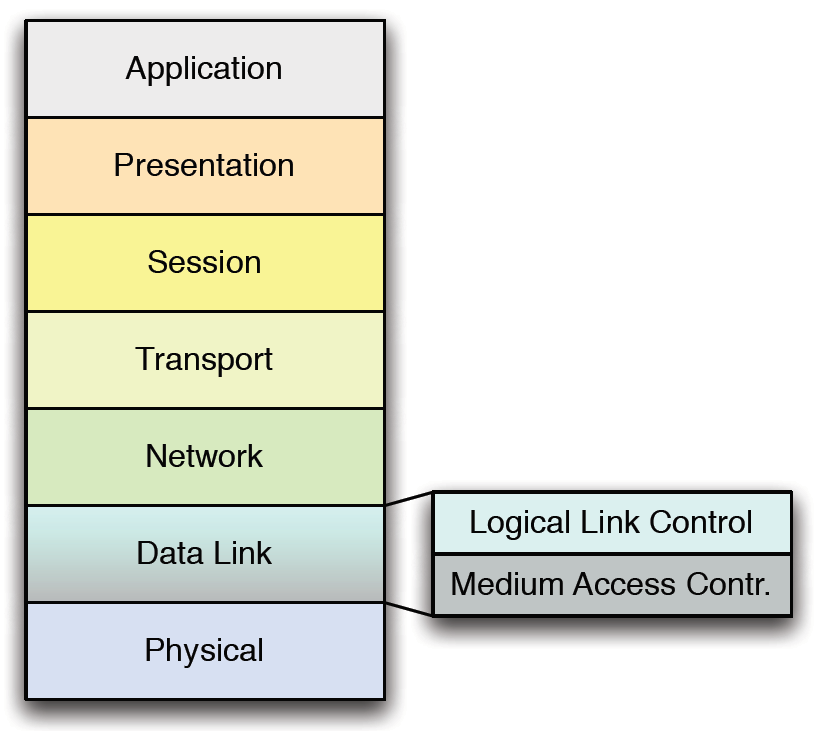
\includegraphics[scale=0.5]{img/isoosi.png}
    \decoRule
    \caption{ISO/OSI architecture.}
    \label{fig:isoosi}
\end{figure}

%-------------------------------------------

\subsection{ISO/OSI protocol stack}
\label{sec:iso_osi}
The \textbf{ISO\footnote{International Organization for Standardization.}/OSI\footnote{Open Systems Interconnection} model} is a conceptual model that characterises and standardises the communication functions of a telecommunication or computing system without regard to its underlying internal structure and technology. Its goal is the interoperability of diverse communication systems with standard communication protocols.

The ISO/OSI model has a seven layer architecture, meaning that it defines seven layers or levels in a complete communication system, as shown in figure \ref{fig:isoosi}. L1-L3 layers are also called \textbf{media layers}, as they are \textit{link-to-link}, while L4-L7 layers are the \textbf{host layers}, because they are end-to-end.

This model \textbf{forbids cross-layer communication} (services that are not tied to a given layer, but may affect more than one layer), even though it would have been useful. The two key principles of the model are:

\begin{itemize}
    \item \textbf{separation of concerns}: functionalities should not be duplicated;
    \item \textbf{information hiding}: implementation should remain hidden and separated from the interface.
\end{itemize}

It is not necessary to develop a separate layer for each and every function outlined in the model. However, by following the general guidelines it provides, developers are able to ensure that a certain level of compatibility is maintained.

%----------------------

\subsubsection*{1. Physical layer}
The \textbf{physical layer} is responsible for the transmission and reception of unstructured raw data between a device and a physical transmission medium. It converts the digital bits into electrical, radio, or optical signals.

%----------------------

\subsubsection*{2. Data Link layer}
The \textbf{data link layer} provides node-to-node data transfer — a link between two directly connected nodes. It detects and possibly corrects errors that may occur in the physical layer. It defines the protocol to establish and terminate a connection between two physically connected devices.

The IEEE 802 divides the data link layer into \textbf{two sublayers}:

\begin{itemize}
    \item \textbf{Medium access control layer} (MAC): responsible for controlling how devices in a network gain access to a medium and permission to transmit data;
    \item \textbf{Logical link control layer} (LLC): responsible for identifying and encapsulating network layer protocols; also controls error checking and frame synchronization.
\end{itemize}

%----------------------

\subsubsection*{3. Network layer}
The \textbf{network layer} provides the functional and procedural means of transferring packets from one node to another connected in different networks.

If the packet (message) is too large to be transmitted from one node to another on the data link layer between those nodes, the network may implement message delivery by splitting it into several fragments at one node, sending the fragments independently, and reassembling them at another node. It may, but does not need to, report delivery errors.

%----------------------

\subsubsection*{4. Transport layer}
The \textbf{transport layer} provides the functional and procedural means of transferring variable length data sequences from a source to a destination host, while maintaining the quality of service functions. It also controls the reliability of a given link through flow control\footnote{\textbf{Flow control} is the process of managing the rate of data transmission between two nodes to prevent a fast sender from overwhelming a slow receiver.}, segmentation/desegmentation, and error control. 

%----------------------

\subsubsection*{5. Session layer}
The \textbf{session layer} controls connections between computers. It establishes, manages (checkpoints, suspends and restarts) and (gracefully) terminates the connections between the local and remote applications.

%----------------------

\subsubsection*{6. Presentation layer}
The \textbf{presentation layer} establishes context between application-layer entities, in which the application-layer entities may use different syntax and semantics if the presentation service provides a mapping between them. If a mapping is available, presentation protocol data units are encapsulated into session protocol data units and passed down the protocol stack. This layer provides independence from data representation by translating between application and network formats. 

%----------------------

\subsubsection*{7. Application layer}
The \textbf{application layer} is the ISO/OSI layer closest to the end user, which means both the ISO/OSI application layer and the user interact directly with the software application. This layer interacts with software applications that implement a communicating component. Such application programs fall outside the scope of the ISO/OSI model. Application-layer functions typically include identifying communication partners, determining resource availability, and synchronizing communication.

%-------------------------------------------

\subsection{TCP/IP protocol stack}
The  \textbf{TCP/IP} stack is  the most commonly used protocol stack throughout the whole Internet. It violates the \textit{separation of concerns} principle of the ISO/OSI model (the truth is that other than being yet another communication stack, ISO/OSI and TCP/IP are two completely different protocols, like the sun and moon).

%----------------------

\subsubsection*{TCP}
Transmission Control Protocol is an Internet protocol suite which breaks up the message into TCP Segments and reassembling them at the receiving side.

%----------------------

\subsubsection*{IP}
An Internet Protocol address that is also known as an IP address is a numerical label. It is assigned to each device that is connected to a computer network which uses IP for communication. Its routing function allows internetworking and essentially establishes the Internet. Combination of IP with a TCP allows developing a virtual connection between a destination and a source.

\begin{figure}[H]
    \centering
    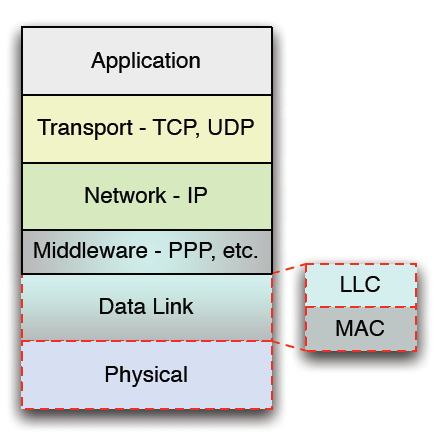
\includegraphics[scale=0.5]{img/tcp.png}
    \decoRule
    \caption{TCP/IP protocol stack architecture.}
    \label{fig:tcp}
\end{figure}

%----------------------

\subsubsection*{1. Data Link layer (L2)}
This layer routes the data between devices on the same network, and manages the exchange of data between the network and other devices. The TCP/IP stack only assumes that the underlying network will do its best to transfer packets from the
source to the destination; no further assumptions are made, so in reality we could use any data link layer (even birds like pigeons, as seen in section \ref{sec:internetmadeof}).

%----------------------

\subsubsection*{2. Network layer (L3)}
At this layer the Internet Protocol (IP) uses the IP address, consisting of a Network Identifier and a Host Identifier, to determine the address of the device it is communicating with.

%----------------------

\subsubsection*{3. Transport layer (L4)}
This is the part of the protocol stack where the Transport Control Protocol (TCP) can be found. TCP works by asking another device on the network if it is willing to accept information from the local device.

%----------------------

\subsubsection*{4. Application layer (L7)}
Protocols for specific functions such as e-mail (Simple Mail Transfer Protocol, SMTP) and file transfer (File Transfer Protocol, FTP) reside at this level.

%-------------------------------------------

\subsection{Addresses}
\textbf{Addresses} are important because, when used incorrectly, they can allow attackers to do lots of bad things: in order to pretend to be somebody else they need a sort of mask, and an address is the best mask behind which an attacker can hide.

%----------------------

\subsubsection{MAC address}
A \textbf{Media Access Control} (\textbf{MAC}) \textbf{address} (also wrongly called \textit{physical address}) is usually a fixed address which has a format (a length) dependent on the technology used by the device's network card.

\vspace{0.5em}

\emph{Example} Ethernet and WiFi devices both have 48-bit MAC addresses; IEEE 802.15.4 has 48-bit or 64-bit MAC address; LTE and other wireless interfaces have different length addresses, and they usually have a particular meaning.

\vspace{0.5em}

The only real requirement for MAC addresses is not that they are unique in the whole Internet, but that there cannot be two different network cards with the same MAC address in the same local network, since the MAC identifies a network card in that specific network.

It is important to note that a card can have more than one MAC address; it depends on the hardware. Usually, most network cards do not allow us to do this, because with more MAC addresses we would be seen in the network as more devices, even though we only have one. Also, there exist hardware devices which can be programmed to filter packets based on more than one MAC address: technically, everything is possible.

Notably, in a network there are also special MAC addresses, like the broadcast address (which directs packets to every network card able to receive it).

By default, when a NIC (network interface controller, another name for what is usually a network card) receives a packet, it checks its header and drops it unless it is addressed to that NIC's MAC address or is a broadcast or multicast addressed packet. In \textbf{promiscuous mode} (a special mode available to all NICs) however, the NIC allows all packets through, thus allowing the computer to read and reply to packets intended for other machines or network devices.

Promiscuous mode can be used in a malicious way to capture private data in transit on a network, so we might be interested in detecting network devices that are in promiscuous mode in order to find potential attackers.

The role of the MAC address is not to prevent this mode; it has been devised for efficiency only: the bus between the NIC and the CPU is a bottleneck, so a network card which is not in promiscuous mode filters all received packets based on their headers and MAC addresses in order to avoid slowing down traffic on the bus with useless packets.

%----------------------

\subsubsection{Numerical address}
\textit{\textbf{Numerical address}} is just another name for \textbf{IP address}, which is necessary for the routing process. It must be compliant with the network we are attached to (meaning that it must be in the range of addresses managed by the router on that network), and it is usually assigned by a network manager. An IP address serves two main functions: \textbf{host identification} and \textbf{location addressing}, and for this reason it must be \textbf{unique} in the global network.

\vspace{0.5em}

\emph{Example} 150.217.8.24 is an IPv4 address, a type of numerical address at layer 3 written in its canonical form.

\vspace{0.5em}

Note that in reality all addresses are binary numbers of a fixed length (32 bits for IPv4 and 128 bits for IPv6). Also, it is possible and perfectly legit for a device to have more than one IP address, for various reasons (for example, if the host is connected to more than one network).

%----------------------

\subsubsection{Alphanumeric address}
Alphanumeric addresses are special addresses that correspond to IP addresses. They are completely free, and their only requirement is that somebody (the DNS) maps them directly and reversely to an IP address, based on a database.

\vspace{0.5em}

\emph{Example} \textit{daconets.dinfo.unifi.it} is an alphanumeric address.

\vspace{0.5em}

In general, a host can have one of more MAC addresses on the same network card, one of more IP addresses for each MAC address, and each IP address can have none, one or more alphanumeric addresses, while on the other hand an alphanumeric address can be mapped to one or more IP addresses (because it consists of a database). However, having one IP mapped to more than one MAC address is not recommended, as lots of bad things can happen. The only case when is a good idea to have this solution is either when being an expert network engineer who attached the device to two different networks, or assigning our IP address to two NICs, one of which is silent.

If an alphanumeric address is mapped to more than one IP address, then it is a responsibility of the source host to choose which one is better, based on either randomness or speed.

%-------------------------------------------

\subsection{IPv4 addressing}
Historically (1980s), IPv4 divided its $2^{32}$ addresses into five different blocks, or \textit{classes}, each for different purposes. The IP address was divided in three parts, the $netID$, $subnetID$ and $hostID$ (see fig. \ref{fig:ipv4classes}), with the $netID$ dependent on the network's class. It was soon observed that this architecture was too complicated and inefficient (routing tables would have been too long), so they were replaced in 1993 by the \textbf{Classless Inter-Domain Routing} (\textbf{CIDR}).

CIDR notation, which takes the form $x.x.x.x/y$ and eliminates the distinction between $netID$ and $subnetID$, is constructed from an IP address, a slash ('/') character, and a decimal number. The trailing number is the count of leading 1-bits (those relevant for the routing process) in the subnet mask. This notation allows the \textit{joining} of addresses differing for their least significant bit. Note that the number of bits of a mask is not necessarily a multiple of a byte (this actually complicates things if we are looking at the address in its canonical form).

If we want to check if two address are in the same subnet (equivalently, if they can be reached directly through the MAC address), then we check if their network parts (those which are specified by the number of bits in the mask) are identical.

\vspace{0.5em}

\emph{Example} The addresses 150.217.8.0/24 and 150.217.9.0/24 differ only for their Least Significant Bit (LSB), so they are joined to form the address 150.217.8.0/23.

\vspace{0.5em}

\emph{Example} 192.168.100.14/24 represents the IPv4 address 192.168.100.14 and its associated routing prefix 192.168.100.0 or, equivalently, its subnet mask 255.255.255.0, which has 24 leading 1-bits.

A 32-bit mask identifies a single host and would have a subnet mask equal to 255.255.255.255, while 24-bit or less masks, like 255.255.255.0, identify networks: the block 192.168.100.0/22 represents the 1024 IPv4 addresses from 192.168.100.0 to 192.168.103.255.

\begin{figure}[H]
    \centering
    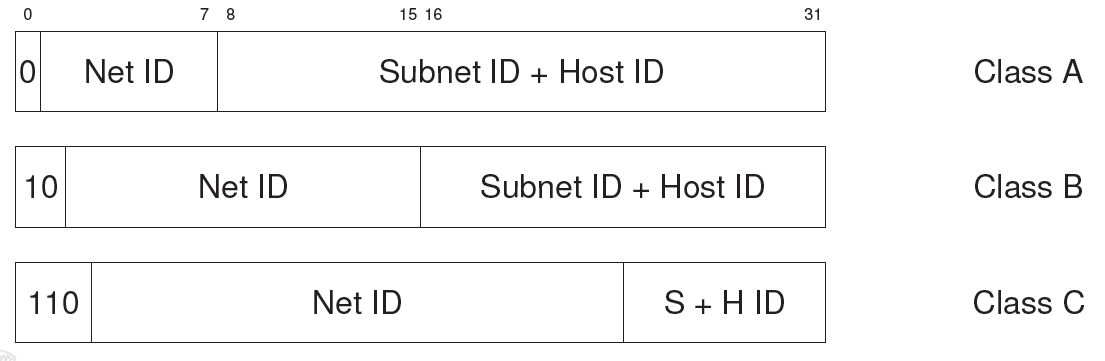
\includegraphics[scale=0.58]{img/ipv4classes.png}
    \decoRule
    \caption{IPv4 classful architecture example; some bits of the $hostID$ are used to code the $subnetID$.}
    \label{fig:ipv4classes}
\end{figure}

%----------------------

\subsubsection{Routing table}
A \textbf{routing table} is a data table stored in a router or a network host that lists the routes to particular network destinations, and metrics (distances) associated with those routes. The routing table contains information about the topology of the network immediately around it. In network security is quite important, as one of the easiest ways to deceive users is to check and take advantage of their routing table.

The routing table consists of at least the following information fields:

\begin{itemize}
    \item \textbf{destination}: the destination IP address, which can be paired with the netmask;
    \item \textbf{netmask} or \textbf{genmask}: the subnet mask that when used together with the destination gives the final network ID, needed for routing;
    \item \textbf{gateway}: also called \textit{next hop}, it is the address of the next station to which the packet is to be sent on the way to its final destination. This is the output interface, which is used in order to send packets outside. An asterisk next to it indicates that it is directly reachable through the current interface, meaning that packets must not pass through the router (otherwise packets will be sent first to the router (gateway));
    \item \textbf{metric}: the routing metric of the path through which the packet is to be sent; the route will go in the direction of the gateway with the lowest metric.
\end{itemize}

Depending on the application and implementation, it can also contain additional values that refine path selection:

\begin{itemize}
    \item \textbf{interface}: identifies the NIC associated with the corresponding network ID (e.g. \textit{eth0} for the first Ethernet card, \textit{eth1} for the second Ethernet card, etc.);
    \item \textbf{QoS flags}: quality of service associated with the route (for example, the U flag indicates that an IP route is up);
    \item \textbf{filtering criteria}: access-control lists associated with the route.
\end{itemize}

\textit{default} is a unique entry in the routing table which indicates the default route (0.0.0.0) and default gateway (which is used whenever there is no specific route in the table for a destination network address).

If two destinations have the same gateway (and the same interface), they are joined together, and the netmask is modified accordingly.

Since we cannot order the routing table in a logical way, in order to find a packet destination we need to find the best match in the routing table. If equation \ref{eq:routing} is true (a bitwise AND operation between the destination address and the netmask, which should be equal to the destination at line $i$), then entry $i$ has a rank equal to the number of 1-bits of $mask_i$; after doing this operation for all entries, we choose the one with the largest rank.

\begin{equation}
\label{eq:routing}
    destIP\; \&\&\; mask_i == destIP_i
\end{equation}

\begin{figure}[H]
    \centering
    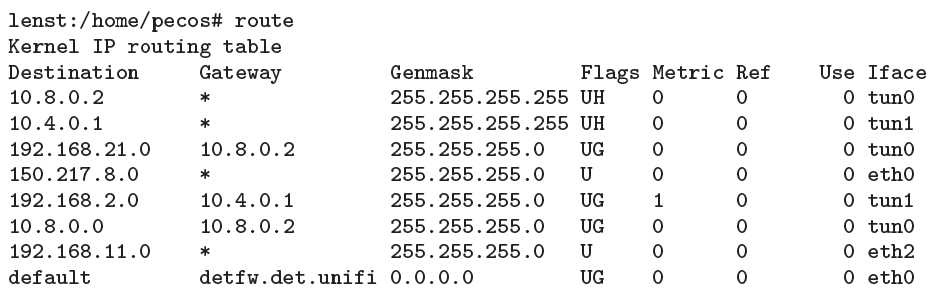
\includegraphics[scale=0.65]{img/routing_table.png}
    \decoRule
    \caption{A computer routing table example.}
    \label{fig:routing_table}
\end{figure}

\vspace{0.5em}

\emph{Example} Figure \ref{fig:routing_table} shows an excerpt from a typical computer routing table. Destination 192.168.21.0 and netmask 255.255.255.0 can be written as network ID 192.168.21.0/24.

This particular routing table has no entry for network 192.168.16.0: if it receives any packets addressed to this network, it will send them via the default gateway.

In general, whoever has the higher number of matching bits wins: suppose we want to route something to 10.8.0.2. We have two lines that match this address in the destination column: 10.8.0.2 (matches for 32 bits) and 10.8.0.0 (matches for 24 bits). The first of these addresses wins and is chosen.

\vspace{0.5em}

%-------------------------------------------

\subsection{Interconnection and data transfer}
Data is exchanged between adjacent nodes as shown in figure \ref{fig:data_transfer}; intermediate nodes should not need to process end-to-end information (except gateways and proxies).

In order to send data, the \textbf{source host} follows these steps:

\begin{enumerate}
    \item Creates a packet directed to the destination host.
    \item Checks if the destination host is in the same subnet as the source by looking at the destination IP (L3) address:
    \begin{itemize}
        \item if it is, the source uses the subnet-specific mechanisms to reach it;
        \item if it is not, the source sends the packet to an appropriate router in its own (the source's) subnet.
    \end{itemize}
    \item The underlying network does the rest (translation of addresses is done here, as this step requires a MAC (L2) address).
\end{enumerate}

Note that alphanumeric addresses have already been resolved, and we work with L3 addresses (IP addresses) from the beginning.

\begin{figure}[H]
    \centering
    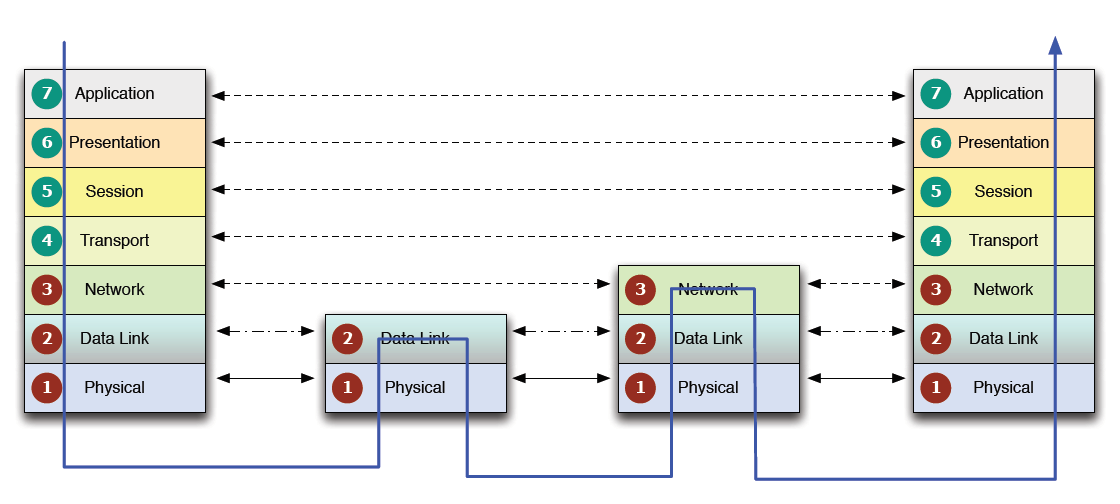
\includegraphics[scale=0.5]{img/data_transfer.png}
    \decoRule
    \caption{Data transfer in the ISO/OSI protocol stack.}
    \label{fig:data_transfer}
\end{figure}